\section{Introduction}

\label{sec:Intro}

% Graph-- Uncertain Graph--Examples 
Graphs are widely used to capture the relationships in emerging applications, such as business to business (B2B) and social networks. 
Sometimes, the existence of the relationship between two entities is uncertain (probabilistic). For instance, in social networks, nodes represent individual users, while edges represent friendship or trust link among them.  Usually, the link strength is derived by inference and prediction models built on interaction details~\cite{Adar_Managing_2007,Kempe_Maximizing_2003}. While edge probability denotes the accuracy of a link prediction or the trust of one person on another. 
In these applications, the data can be modeled and shared as uncertain graphs whose edges carries a probability of existence. The probability represents the confidence that the relationship holds in reality. 

\begin{figure}[!htb]
    \subfigure[Social Trust Network]{\label{fig:socialNetwork}
      \begin{minipage}[l]{0.45\columnwidth}
        \centering
        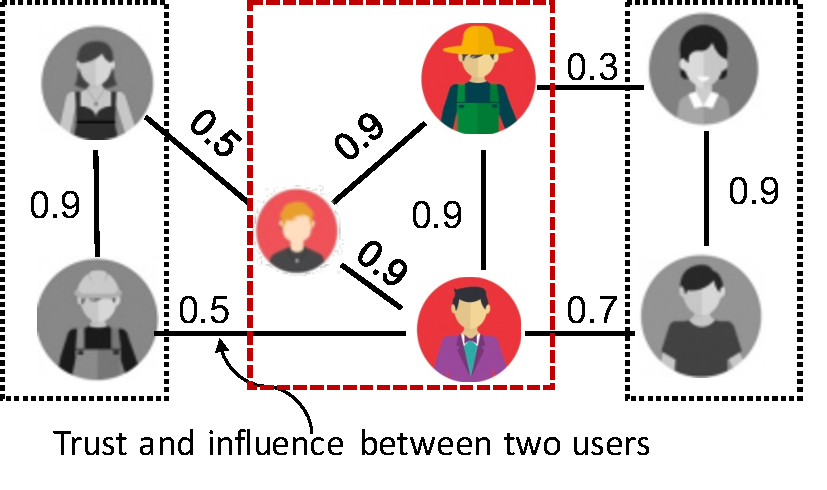
\includegraphics[height=2.3cm]{ill/SocialNetwork.pdf}
      \end{minipage}
      }
    \subfigure[B2B Network]{\label{fig:b2bNetwork}
      \begin{minipage}[l]{0.45\columnwidth}
        \centering
        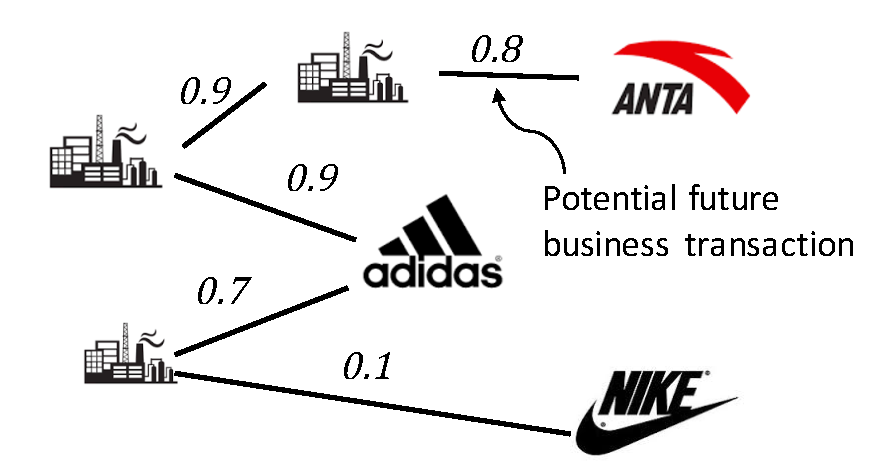
\includegraphics[height=2.3cm]{ill/B2BNetwork.pdf}
      \end{minipage}
      }
    \vspace{-6pt}
    \caption{Real-world uncertain graphs with privacy concerns.}
    \label{fig:motivation}
    \vspace{-10pt}
\end{figure} 

% Sharing--Privacy--Examples 
These uncertain graphs are invaluable for scientific research and commercial applications e.g., understanding social interactions, information propagation and advertising~\cite{Kempe_Maximizing_2003,Cho_Friendship_2011}. 
Compared to sharing the results of graph mining, graph sharing gives greater flexibility as recipients can perform unlimited analysis, data explosion with novel methods.

However, sharing these uncertain graphs could seriously jeopardize the privacy of users or entities profiled inside.
In social trust network, the trust relationships among users, which significantly impact users' behaviors, are usually probabilistic.  They are useful in social interaction study and micro-targeting~\cite{Kempe_Maximizing_2003}. However, users are unwilling to share such confidential information with potential adversaries. In B2B networks, business operators also hesitate to share transaction patterns as it relates to confidential business models. Such tension is raising the question of sharing uncertain graphs without compromising privacy. 

% State-of-Art %
A number of privacy preserving graph sharing schemes have been studied in the deterministic scenario~\cite{Liu_Towards_2008,Ying_Randomizing_2008,Wang2011,Liu_Privacy_2009,Nguyen_Anonymizing_2015,Sala_Sharing_2011,Xiao_Differentially_2014,lee2011}, though many problems still remain unexplored in the uncertain scenario.
\begin{figure}[!htb]
  \centering
  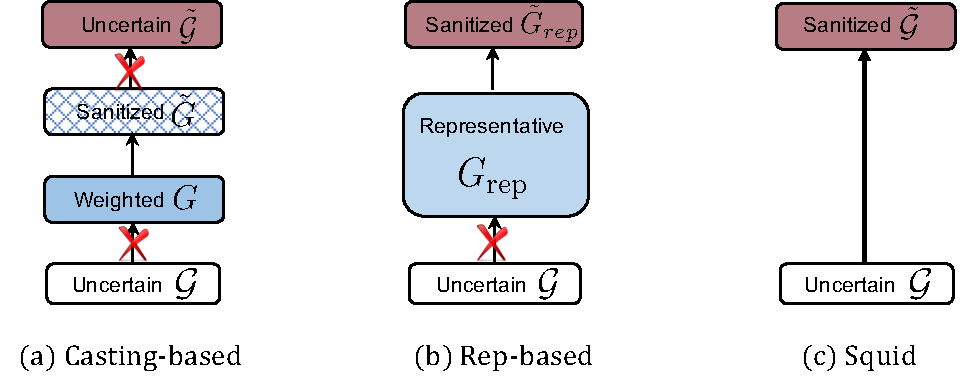
\includegraphics[width=0.9\linewidth]{ill/methods.pdf}
  \caption{Illustration of three anonymization approaches.}
\end{figure}

An obvious approach is to convert the uncertain graph sharing problem into the deterministic one by casting edge probabilities as edge weights. 
While, the general idea is appealing, the casting-based method is inadequate to provide desirable utility for uncertain graph. 
By disregarding the possible world semantics of the uncertain graph, casting-based approach, as later illustrated, fails to reflect uncertain graph properties such as connectivity, dense subgraphs correctly~\cite{Zhao_Detecting_2014,Hua_Probabilistic_2010}. 
Hence, the casting-based scheme could produce poor results in the uncertain scenario even if the weighted graph anonymization algorithm is good. 

\textbf{Example}. \emph{Connectivity of deterministic subgraphs is generally measured by the concept of cut, which is defined as the sum of weights of intra edges. Generally, the bigger the cut, the harder to separate two subgraphs. In Figure~\ref{fig:motivation}(a), the equal cut $C(SG_{1},SG_{2})=C(SG_{3},SG_{2})=1$ implies the identical connectivity of $SG_{1}$ and $SG_{3}$ {\wrt} $SG_{2}$. However, with the possible world semantics, we know the probability to separate $SG_{1}$ and $SG_{2}$ is $(1-0.5)^{2}=0.25$, and that to separate $SG_{2}$ and $SG_{3}$ is $(1-0.3)(1-0.7)=0.21$. Hence, in fact, $SG_{2}$ is closer to $SG_{1}$ than to $SG_{3}$. }

In the previous work~\cite{Xiao:2018}, we ever proposed a representative-based method, based on the idea of processing uncertain graph through representative instances~\cite{Parchas_Gullo_Papadias_Bonchi_2014}.
It first extracts a single deterministic representative instance $G$ that capture structural properties of the uncertain graph.
After that, anonymization can then proceed efficiently on $G$ using conventional algorithms, regardless of the uncertainty.  
The advantage of this method is that it does not require new anonymization techniques. 
However, the representative-based method is not always feasible. 
The detachment of edge uncertainty deteriorates the data utility. 

As ever discussed, conventional graph anonymization schemes are inadequate to share uncertain graphs with a desirable trade-off between privacy and utility. 
It is worthwhile to consider developing the specially optimized solution for handling following challenges. 

$\bullet$~\textup{\emph{Stochastic Privacy Attacks.}}~~Edge uncertainty plays an indispensable role in the uncertain graph model. Discarding them in the release is impractical.  
However, the extra release of edge uncertainty makes privacy protection far more difficult as it empowers the adversary and makes the profiled entity more vulnerable. 
To this end, we clarify the potential re-identification attack and adopt a privacy notion for releasing privacy-preserving uncertain graphs.

$\bullet$~\textup{\emph{Stochastic Utility Loss Metric.}}~~It is challenging to maintain the structure when the uncertain graph is modified to pursue anonymity. 
The structural distortion incurred is evaluated by the specially designed utility loss metric.  
It aims to safeguard the utility of the release graphs.  
Unfortunately, current graph utility loss metrics such as graph edit distance~\cite{Liu_Towards_2008}, spectrum discrepancy~\cite{Ying_Randomizing_2008}, community reconstruction error~\cite{Wang2011} and shortest path discrepancy~\cite{Liu_Privacy_2009} 
are not suitable in our problem setting because of the ignorance of edge uncertainty.
In this context, the discrepancy w.r.t the uncertain graph reliability becomes a useful criterion. It evaluates the connectivity difference in the context of the entire graph and meanwhile utilizes the possible world semantics. 

$\bullet$~\textup{\emph{Intractable Search Space.}}~~Informally, our goal is to find a sanitized graph with the desired level of privacy with as few graph mutations as possible. 
Even the simple deterministic graph anonymization problem, {\ie}, is known to be NP-hard when mutations are limited to edge additions and deletions~\cite{Hartung_Theory_2015}. 
In the probabilistic scenario, edge modifications are no longer limited to edge addition and deletion, but can be infinite probability deviations. 
Exhaustive search is computationally intractable if the number of edges is large. 
It makes the uncertain graph anonymization problem very challenging. 
In this work, we approximate the problem of interest via a randomized algorithm, which built on the basis of meta-heuristics. 

In this work, we propose a novel sanitization solution tailored towards uncertain graphs via incorporating possible world semantics and test it on three real-life network datasets. We analyze the utility of sanitized graphs (uncertain ones) in two scenarios: extracting statistics for graph analysis, and performing influence prorogation. We show our method preserves as much the stochastic nature of the original uncertain graph as possible while injecting necessary structural noise to guarantee a desirable level of privacy. We also show that significant improvement of our methods over casting-based and representative-based methods. 
Specifically, we make the following contributions.
\begin{itemize}
\item We are the first to formulate the uncertain graph sharing problem. 
 We show the potential re-identification attack and present a practical privacy notion. 
\item Motivated by the use of connectivity error, we propose a utility loss metric on the basis of reliability. It evaluates the connectivity difference in the context of the entire graph and also utilizes the possible world model. 
\item To alleviate the combinational intractability, we propose a randomized algorithm boosted by the hybrid of uncertainty-aware heuristics. It excels in identifying a population of sanitized results with good quality efficiently.
\item We conduct extensive experimental studies to demonstrate efficiency and practical utility of our algorithms. The results demonstrate a significant advantage over the conventional methods that do not directly consider edge uncertainties.
\end{itemize}

The rest of the paper is organized as follows. In Section~\ref{sec:relatedWork}, we summarize related works, point out the limitation of existing methods, and clarify our distinct privacy goal. In Section~\ref{sec:notation} we formulate the uncertain graph-anonymization problem. Sections~\ref{sec:soa} –~\ref{sec:method} present our anonymization approach for releasing privacy-preserving uncertain graph.  In Section~\ref{sec:ex} we apply our method to several real-world uncertain graphs and demonstrate its performance, practical utility and efficiency. 